%You can switch between the two styles in order to create slides or handouts
\documentclass[fleqn]{beamer}
%\documentclass[handout]{beamer}

\usepackage{amsmath,amssymb,amsfonts} % mathematical and other special symbols and fonts
\usepackage{tikz} % support for drawing graphs and diagrams
\usetikzlibrary{arrows,decorations.pathmorphing,positioning,fit,trees,shapes}
\usepackage{xcolor} % color support
\usepackage{hyperref} % hyperlink support (also internal links)
\usepackage{listings} % listings and \lstinline support for code typesetting
\lstset{language=C++}
%\usepackage[english]{babel} % needed for English texts (translations, e.g. References --> Literatur)

\usepackage[utf8x]{inputenc} % unicode encoding
\usepackage{graphicx} % support for \includegraphics{}

\usepackage{mathtools}
\usepackage{amsthm}
\usetheme{Hybrid}
\usepackage{lmodern}
\usetheme{Luebeck}
\usepackage{lipsum} % <= to insert dummy text
\usepackage[absolute,overlay]{textpos}
\usetikzlibrary{arrows,positioning}




\setbeamercolor*{block title example}{fg=blue!50,
bg= blue!10}
\setbeamercolor*{block body example}{fg= blue,
bg= blue!5}

\setbeamertemplate{navigation symbols}{}   

\title{SMT for Strings}
\subtitle{Seminar: Satisfiability Checking}
\author[Meshkatul Anwer]{Meshkatul Anwer\\ \small{Supervision: Cornelius Aschermann}}
\institute[THS]{}
\date{SS 2015}
%\titlegraphic{\includegraphics[scale=0.3]{hybrid_logo}}
\titlegraphic{\includegraphics[scale=0.15]{rwth}}

\begin{document}

\frame{\titlepage}%creates titlepage 

\frame{
  \frametitle{Introduction}  
\begin{itemize}
\item Web service security is important.
\item String is the main information carrier.  
\item String reasoning is important.  
\item Here we will present : SMT for strings.
\end{itemize}
}

\frame{
  \frametitle{Objectives}  
\begin{itemize}
\item We want a string solver: 
	\begin{itemize}
		\item Fast
		\item Robust
        \item Expressive(Regexp)
        \item Other Theories (Int, Bool)        		
	\end{itemize}
\end{itemize}
}

\frame{
  \frametitle{Constraints:examples}  
  
\begin{itemize}
\item The language for $\mathcal{T}_{SL}$: 
	\begin{itemize}
        \item over a finite set of alphabets $\mathcal{A}$ (e.g. 256 ASCII characters)     
		\item terms can be \underline{constants} e.g. \texttt{"a"}, \texttt{"ab"}, \texttt{"abc"},\texttt{"helloWorld"}, ...
		\item terms can be free \underline{constants} or \underline{variables} ( e.g. \texttt{x}, \texttt{y}, \ \texttt{z},... )
		\item terms can be String concatenation: $\texttt{con}:String  \times \cdots \times String \to String$   
		\item terms can be length terms: $\texttt{len}: String \to Int$   
	\end{itemize}
\end{itemize}
}

\frame{
  \frametitle{Constraints:examples}  
\begin{itemize}
\item examples of String constraints: 
	\begin{itemize}
	    \item $s_1: \texttt{x} =  \texttt{con}(\texttt{"ab"}, \texttt{z}) $   
        \item $s_2: \texttt{y} =  \texttt{con}(\texttt{"de"}, \texttt{z}) $   
        \item $s_3: \texttt{y} =  \texttt{con}(\texttt{"abc"}, \texttt{l})$   
        \item $s_4: \texttt{x} =  \texttt{y}$   \pause
	\end{itemize}
\end{itemize}

\begin{itemize}
\item example of length constraints: 
	\begin{itemize}
	    \item $s_5: \texttt{len} (\texttt{x}) > 6$
	\end{itemize}
\end{itemize}

		\begin{itemize}
  		\item example of the Boolean formula: 
  			\begin{itemize}
  			    \item $ assert (s_1 \wedge (s_2 \vee s_3 ) \wedge s_4 \wedge s_5)$ 
  			\end{itemize}
  		\end{itemize}

}
\begin{frame}[fragile]
  \frametitle{Constraints:encoding into smtlib} 

\begin{textblock*}{40mm}(85mm,9mm)
\tiny
\begin{exampleblock}{}
  constraints:
  	\begin{itemize}
  	\setlength\itemsep{0.1em}
  	    \item $s_1: \texttt{x} =  \texttt{con}(\texttt{"ab"}, \texttt{z}) $   
        \item $s_2: \texttt{y} =  \texttt{con}(\texttt{"de"}, \texttt{z}) $   
        \item $s_3: \texttt{y} =  \texttt{con}(\texttt{"abc"}, \texttt{l})$   
        \item $s_4: \texttt{x} =  \texttt{y}$   
   	    \item $s_5: \texttt{len} (\texttt{x}) > 6$
  	\end{itemize}
  	formula:
		\begin{itemize}
  		   \item $ assert (s_1 \wedge (s_2 \vee s_3 ) \wedge s_4 \wedge s_5)$
  		\end{itemize}
\end{exampleblock}
\end{textblock*}


\begin{figure}[width=5cm]
\scriptsize
\begin{lstlisting}
(set-option:produce-models true)
(set-logic QF_S)
 
(declare-fun x () String)
(declare-fun y () String)
(declare-fun z () String)
(declare-fun l () String)
 
(assert (= x (str.++ "ab" z)))
(assert (or (= y (str.++ "de" z)) (= y (str.++ "abc" l))) )
(assert (=  x  y)) 
(assert (> (str.len x) 6)) 
 
(check-sat)
(get-value (x y z l) )	
\end{lstlisting}

\caption{ \scriptsize the formula encoded in smt-lib 2 format}
\end{figure}\pause

\begin{figure}[h]
\includegraphics[width=12cm]{cvc_output.png}
\caption{ \scriptsize the output from cvc4}
\end{figure}
\end{frame}
\frame{
  \frametitle{Introduction to CVC4}  
  \begin{itemize}
  \item CVC4 
	\begin{itemize}
		\item CVC4 is an automatic theorem prover for Satisfiability Modulo Theories.
		\item along with other theories it also supports 'Theory of Strings'. 
		\item the theory solver for strings is implemented as natively.
	\end{itemize}  
  \item Features:
  	\begin{itemize}  		
        \item allows constraints with unbounded Strings, 
  		\item does not translate the problem into other theories (e.g. bitvectors)
		\item the procedure is algebraic in approach. 
  	\end{itemize}
  \end{itemize}

}

\frame{
  \frametitle{Overview of the procedure}  
  \begin{itemize}
    \item The procedure is defined as a set of derivation rules.
    \item The repeated application of rules produces a derivation tree, where each node in the derivation tree is called a \underline{$configuration$}.
    \item while the rule application, the tree splits with new configuration, where
    \begin{description}
        \item[-] no further rule application is possible
        \item[-] or the configuration is \texttt{unsat}, then backtrack and take another branch if exists        
      \end{description}
    \item If the procedure ends up with a \underline{$closed$} tree, then it concludes as \texttt{unsat}.
    \item or If the procedure ends up with a \underline{$saturated$} configuration, then it concludes as \texttt{sat}.    
  \end{itemize}
}


\frame{
  \frametitle{Procedure}  
  The main procedure is based on the repeated application of the rules according to the following steps,
  \begin{enumerate}
    \item $Check\ conflicts$ 
    \item $Propagate$
    \item $Split\ by Length$
    \item $Normalize$
    \item $Partition$
    \item $Check\ cardinality$
  \end{enumerate}
  
  Note:
    \begin{itemize}
      \item $S:$ set of string constraints.
      \item $A:$ set of arithmetic constraints.
    \end{itemize}
  
}

\frame{
  \frametitle{Procedure: Step 0:$Start\ of\ the\ procedure$}

\begin{textblock*}{41mm}(100mm,-5mm)
\tiny
\begin{exampleblock}{}
  	\begin{enumerate}
  	\setlength\itemsep{0.1em}
  	        \item $Check\ conflicts$ 
  	        \item $Propagate$
  	        \item $Split\ by\ Length$
  	        \item $Normalize$
  	        \item $Partition$
  	        \item $Check\ cardinality$  	    
  	\end{enumerate}
\end{exampleblock}
\end{textblock*}

  \begin{itemize}
    \item This is the start of the procedure. \begin{figure}
\begin{align*}
\texttt{con}(\mathbf{s},  \texttt{con}(\mathbf{t}), \mathbf{u}) &\rightarrow   \texttt{con}(\mathbf{s},\mathbf{t}, \mathbf{u})\\
\texttt{con}(\mathbf{s}, \epsilon, \mathbf{u}) &\rightarrow \texttt{con}(\mathbf{s}, \mathbf{u})\\
\texttt{con}(s) &\rightarrow s\\
\texttt{con}() &\rightarrow \epsilon\\
\texttt{con}(\mathbf{s}, c_1 \cdots c_i, c_{i+1} \cdots c_n, \mathbf{u}) &\rightarrow \texttt{con}(\mathbf{s}, c_1 \cdots c_n, \mathbf{u})\\
\texttt{len}( \texttt{con}(s_1,\cdots,s_n)) &\rightarrow \texttt{len}(s_1) + \cdots + \texttt{len}(s_n)\\
\texttt{len}(c_1,\cdots,c_n) &\rightarrow n
\end{align*}
\end{figure}
    \item All the terms must be in normalized form, according to the above reduction rules.
  \end{itemize}
        \begin{description}
          \item e.g. $\texttt{con}("ab", \texttt{con}("c", l)) \rightarrow \texttt{con}("abc",l) $
          \item e.g. $\texttt{len}("abc") \rightarrow 3$
          \item e.g. $\texttt{len}(\texttt{con}("abc", "def"))\rightarrow 6$
        \end{description}
}

\frame{
  \frametitle{Procedure: Step 1:$Check\ conflicts$}

\begin{textblock*}{41mm}(100mm,-5mm)
\tiny
\begin{exampleblock}{}
  	\begin{enumerate}
  	\setlength\itemsep{0.1em}
  	        \item \underline{$Check\ conflicts$} 
  	        \item $Propagate$
  	        \item $Split\ by\ Length$
  	        \item $Normalize$
  	        \item $Partition$
  	        \item $Check\ cardinality$  	    
  	\end{enumerate}
\end{exampleblock}
\end{textblock*}

  \begin{itemize}
    \item Check is there any contradiction exists in the current \\constraints
    \item Rules used: \texttt{S-Conflict} , \texttt{A-Conflict}.
    \begin{figure}
\begin{align*}
 \texttt{A-Conflict} &\frac{ A \models_{LIA} \perp }{ \textnormal{unsat}}\\  
 \texttt{S-Conflict} &\frac{ s\approx t \in S \ \ s \not\approx t \in S}{\textnormal{unsat}}
\end{align*}
\end{figure}
    \item Examples: 
      \begin{itemize}
          \item e.g. $S:\{ \cdots, x \approx \epsilon,x\not\approx \epsilon, \cdots\} \rightarrow{\texttt{unsat}}$      
          \item e.g. $S:\{ \cdots, x \approx y,x\not\approx y, \cdots\} \rightarrow{\texttt{unsat}}$      
          \item e.g. $A:\{ \texttt{len}(x) \approx \texttt{len}(y), \texttt{len}(x) \not\approx \texttt{len}(y) \}\rightarrow{\texttt{unsat}}$      
       \end{itemize} 
  \end{itemize}
}

\frame{
  \frametitle{Procedure: Step 2:$Propagate$}

\begin{textblock*}{41mm}(100mm,-5mm)
\tiny
\begin{exampleblock}{}
  	\begin{enumerate}
  	\setlength\itemsep{0.1em}
  	        \item $Check\ conflicts$ 
  	        \item \underline{$Propagate$}
  	        \item $Split\ by\ Length$
  	        \item $Normalize$
  	        \item $Partition$
  	        \item $Check\ cardinality$  	    
  	\end{enumerate}
\end{exampleblock}
\end{textblock*}

  \begin{itemize}
    \item Introduce new constraints induced by constraints of other theories \\(e.g. $\mathcal{T}_{LIA}$ and $\mathcal{T}_{SL} $).  
    \item Rules used : \texttt{S-Prop}, \texttt{A-Prop}.
    \begin{figure}
    \begin{align*}
 \texttt{A-Prop} &\frac{ S \models  \texttt{len} \ x \approx \texttt{len} \ y}{ A := A, \texttt{len} \ x \approx \texttt{len} \ y}\\
  \texttt{S-Prop} &\frac{ A \models_{LIA}  \texttt{len} \ x \approx \texttt{len} \ y}{ S := S, \texttt{len} \ x \approx \texttt{len} \ y}
      \end{align*}
    \end{figure}    
    
    \item Examples: 
      \begin{itemize}
          \item e.g. $S \models (\texttt{len} \ x \approx \texttt{len} \ y) \rightarrow A:=A,{\texttt{len} \ x \approx \texttt{len} \ y}$      
          \item e.g. $S \models (\texttt{len} \ x \approx \texttt{len} \ "abc") \rightarrow A:=A,{\texttt{len} \ x = 3 }$      
       \end{itemize} 
  \end{itemize}
}

\frame{
	\frametitle{Procedure: Step 3:$Split\ by\ Length$}
	
	\begin{textblock*}{41mm}(100mm,-5mm)
	\tiny
	\begin{exampleblock}{}
	  	\begin{enumerate}
	  	\setlength\itemsep{0.1em}
	  	        \item $Check\ conflicts$ 
	  	        \item $Propagate$
	  	        \item \underline{$Split\ by\ Length$}
	  	        \item $Normalize$
	  	        \item $Partition$
	  	        \item $Check\ cardinality$  	    
	  	\end{enumerate}
	\end{exampleblock}
	\end{textblock*}
	
	\begin{itemize}
     	\item Introduce new constraint into the set of arithmetic \\constraints for equalities in string constraints.
     	\item Introduce branching for free variables in string constraints.
		\item Rules used: \texttt{Len} and \texttt{Len-Split}.
		
		\begin{figure}
			\begin{align*} 
			\texttt{Len} &\frac{ x \approx t \in \mathcal{C}(S) \ x \in \mathcal{V}(S)}{ A := A, \texttt{len} \ x \approx (\texttt{len} \ t) \downarrow}\\
			%\texttt{Len-Split} &\frac{ x \in \mathcal{V}(S \cup A) \ x: Str}{ S := S, x \approx \epsilon \parallel  A:= A, \texttt{len} \ x > 0}
			\end{align*}
		\end{figure}    
		
		\item Examples: 
		\begin{itemize}
			\item e.g. $S \models (x \approx y) \rightarrow A:=A,{\texttt{len} \ x \approx \texttt{len} \ y}$      
			\item e.g. $S \models (x \approx "abc") \rightarrow A:=A,{\texttt{len} \ x = 3 }$      
		\end{itemize} 
	\end{itemize}
}


\frame{
	\frametitle{Procedure: Step 4:$Normalize$}
	
	\begin{textblock*}{41mm}(100mm,-5mm)
	\tiny
	\begin{exampleblock}{}
	  	\begin{enumerate}
	  	\setlength\itemsep{0.1em}
	  	        \item $Check\ conflicts$ 
	  	        \item $Propagate$
	  	        \item $Split\ by\ Length$
	  	        \item \underline{$Normalize$}
	  	        \item $Partition$
	  	        \item $Check\ cardinality$  	    
	  	\end{enumerate}
	\end{exampleblock}
	\end{textblock*}
	
	\begin{itemize}
		\item Compute the normalized form for each term. 
		\item If there is term not in normalized, apply splitting and then finally unify. 
		\item Rules used: \texttt{S-Cycle}, \texttt{L-Split}, \texttt{F-Unify}		
		\begin{figure}
			\scriptsize
			\begin{align*}
			\texttt{F-Unify} &\frac
			{ F \ s = ( w,u,u_1) \ \ F \ t = (w, u,v_1) \  s\approx t \in \mathcal{C}(S) \ S \models \textnormal{len} \ u \approx \textnormal{len} \ v }
			{ S:= S, u \approx v}
			\end{align*}
		\end{figure}    
		
		\item Examples: 
		\begin{itemize}
			\item e.g. $\texttt{con}(x, m) \approx \texttt{con}(y, n) , \texttt{len}(x) \approx \texttt{len}(y)  \rightarrow S:=S,{ x \approx  y}$
		\end{itemize} 
	\end{itemize}
}


\frame{
	\frametitle{Procedure: Step 5:$Partition$}
		\begin{textblock*}{41mm}(100mm,-5mm)
		\tiny
		\begin{exampleblock}{}
		  	\begin{enumerate}
		  	\setlength\itemsep{0.1em}
		  	        \item $Check\ conflicts$ 
		  	        \item $Propagate$
		  	        \item $Split\ by\ Length$
		  	        \item $Normalize$
		  	        \item \underline{$Partition$}
		  	        \item $Check\ cardinality$  	    
		  	\end{enumerate}
		\end{exampleblock}
		\end{textblock*}
	
	
	\begin{itemize}
		\item Each equivalence class should be in their corresponding group (bucket).
		\item If the partition is not compete, apply splitting on the free variables.
		\item Rules used: \texttt{D-Base}, \texttt{D-Add}, \texttt{S-Split} and \texttt{L-Split}. 		
		\begin{figure}
			\scriptsize
			\begin{align*}
			            \texttt{S-Split} &\frac
						{ x, y \in \mathcal{V}(S) \ \ x \approx y, x \not\approx y \in \mathcal{C}(S) }
						{ S := S, x \approx y \parallel S:= S, x \not\approx y}\\
						\texttt{L-Split} &\frac
						{ x, y \in \mathcal{V}(S) \ \ x,y: \textnormal{Str}  \ \  S \not\models \texttt{len} \ x \not\approx \textnormal{len} \ y}
						{ S:= S, \textnormal{len} \ x \approx \texttt{len} \ y \parallel S:=S, \textnormal{len} \ x \not\approx \texttt{len} \ y}
			\end{align*}
		\end{figure}   		
	\end{itemize}
}
\frame{
	\frametitle{Procedure: Step 6:$Check\ cardinality$}
	
		\begin{textblock*}{41mm}(100mm,-5mm)
		\tiny
		\begin{exampleblock}{}
		  	\begin{enumerate}
		  	\setlength\itemsep{0.1em}
		  	        \item $Check\ conflicts$ 
		  	        \item $Propagate$
		  	        \item $Split\ by\ Length$
		  	        \item $Normalize$
		  	        \item $Partition$
		  	        \item \underline{$Check\ cardinality$}  	    
		  	\end{enumerate}
		\end{exampleblock}
		\end{textblock*}
	
	\begin{itemize}
		\item For each bucket $B$ introduce new an arithmetic constraint, as the alphabet $\mathcal{A}$ is finite.
		\item Performed as a last step of the procedure.		
		\item For example, 
		 \begin{itemize}
		 	\item If
		    \begin{itemize}
				\item we have 256 characters, and
				\item $S$ entails that 257 distinct strings of length 1 exist 
		    \end{itemize}
		    \item Then \begin{itemize}
				\item $S$ is unsatisfiable
			\end{itemize}
		\end{itemize}	  

	\end{itemize}
}
\frame{
	\frametitle{Derivation Tree Example }
\begin{textblock*}{40mm}(85mm,9mm)
\tiny
\begin{exampleblock}{}
  constraints:
  	\begin{itemize}
  	\setlength\itemsep{0.1em}
  	    \item $s_1: \texttt{x} =  \texttt{con}(\texttt{"ab"}, \texttt{z}) $   
        \item $s_2: \texttt{y} =  \texttt{con}(\texttt{"de"}, \texttt{z}) $   
        \item $s_3: \texttt{y} =  \texttt{con}(\texttt{"abc"}, \texttt{l})$   
        \item $s_4: \texttt{x} =  \texttt{y}$   
   	    \item $s_5: \texttt{len} (\texttt{x}) > 6)$
  	\end{itemize}
  	formula:
		\begin{itemize}
  		   \item $ assert (s_1 \wedge (s_2 \vee s_3 ) \wedge s_4 \wedge s_5)$
  		\end{itemize}
\end{exampleblock}
\end{textblock*}
	
	\begin{figure} 	
		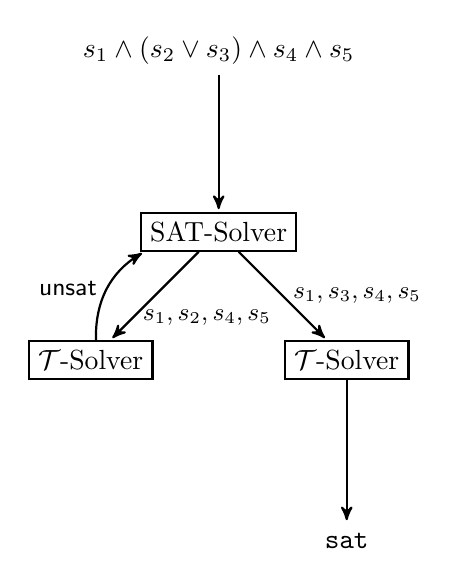
\begin{tikzpicture}[->,>=stealth',
		shorten >=1pt,auto,node distance=2.3cm,thick,
		main node/.style={rectangle,draw}, text node/.style={rectangle}]
		
		\node (root) {$ s_1 \wedge (s_2 \vee s_3 ) \wedge s_4 \wedge s_5$};
		\node[main node] (sat-solver) [below of=root] {SAT-Solver};
		\node[main node] (t-solver-1) [below left of=sat-solver] {$\mathcal{T}$-Solver};
		\node[main node] (t-solver-2) [below right of=sat-solver] {$\mathcal{T}$-Solver};	
		\node[text node] (sat) [below of=t-solver-2] {$ \texttt{sat}$};
		
		
		\path[every node/.style={font=\sffamily\small}]
		(root) edge node [left] {} (sat-solver)	
		
		(sat-solver) edge node [right, near end] { $s_1 ,s_2 ,  s_4, s_5$} (t-solver-1)
		(sat-solver) edge node [right] {$s_1 ,s_3 ,  s_4, s_5$} (t-solver-2)	
		(t-solver-1) edge [bend left] node [left] {unsat} (sat-solver)	
		(t-solver-2) edge  node [right] {} (sat);
		\end{tikzpicture}			
	\end{figure}	
}

\frame{
	\frametitle{Left derivation tree }
	\begin{textblock*}{40mm}(85mm,0mm)
		\tiny
		\begin{exampleblock}{}
			constraints:
			\begin{itemize}
				\setlength\itemsep{0.1em}
				\item $s_1: \texttt{x} =  \texttt{con}(\texttt{"ab"}, \texttt{z}) $   
				\item $s_2: \texttt{y} =  \texttt{con}(\texttt{"de"}, \texttt{z}) $   
				\item $s_3: \texttt{y} =  \texttt{con}(\texttt{"abc"}, \texttt{l})$   
				\item $s_4: \texttt{x} =  \texttt{y}$   
				\item $s_5: \texttt{len} (\texttt{x}) > 6)$
			\end{itemize}
			formula:
			\begin{itemize}
				\item $ assert (s_1 \wedge (s_2 \vee s_3 ) \wedge s_4 \wedge s_5)$
			\end{itemize}
		\end{exampleblock}
	\end{textblock*}
	
	\begin{figure} 	
		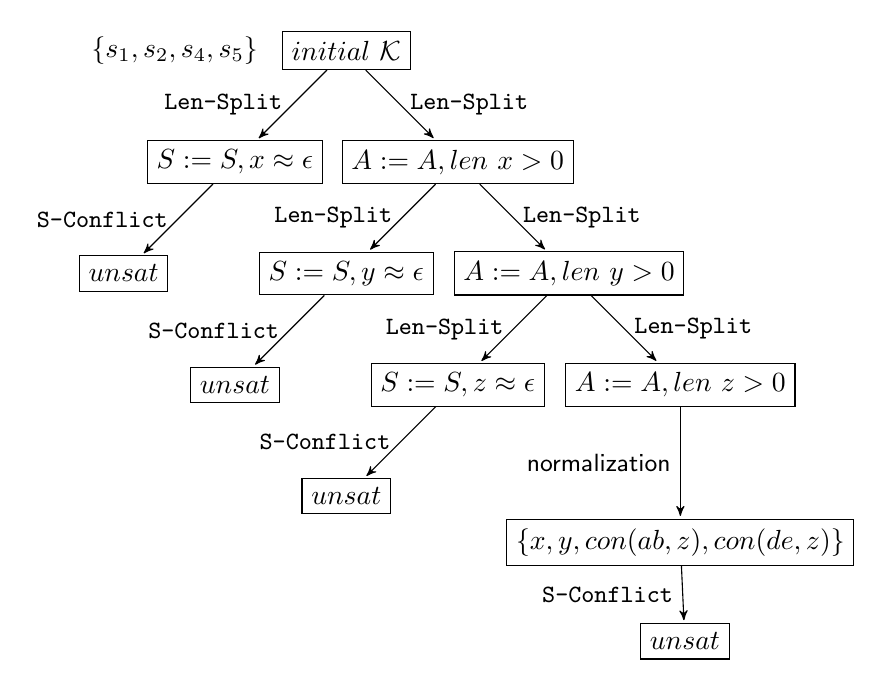
\begin{tikzpicture}[->,>=stealth',
		shorten >=1pt,auto,node distance=2cm,thin,
		main node/.style={rectangle,draw}, text node/.style={rectangle}]
		
		
		\node [left] at (-10mm,0) {$ \{s_1, s_2, s_4,  s_5\}$};
		\node[main node] (a) {$initial\ \mathcal{K}$};
		\node[main node] (b) [below left of=a] {$S:=S, x\approx \epsilon$};
		\node[main node] (c) [below right of=a] {$A:=A, len\ x > 0$};
		
		\node[main node] (d) [below left of=b] {$unsat$};
		\node[main node] (e) [below left of=c] {$S:=S, y\approx \epsilon$};
		\node[main node] (f) [below right of=c] {$A:=A, len\ y > 0$};
		
		\node[main node] (g) [below left of=e] {$unsat$};
		\node[main node] (h) [below left of=f] {$S:=S, z\approx \epsilon$};
		\node[main node] (i) [below right of=f] {$A:=A, len\ z > 0$};
		
		\node[main node] (j) [below left of=h] {$unsat$};
		\node[main node] (k) [below of=i] {$\{ x,y,con(ab,z),con(de,z)\}$};
		
		\node [draw] (l) at (43mm,-75mm)  {$unsat$};
		
		
			\path[every node/.style={font=\sffamily\small}]
			(a) edge node [left] {\texttt{Len-Split}} (b)
			(a) edge node [right] {\texttt{Len-Split}} (c)
			(b) edge node [left] {\texttt{S-Conflict}} (d)
			(c) edge node [left] {\texttt{Len-Split}} (e)
			(e) edge node [left] {\texttt{S-Conflict}} (g)
			(c) edge node [right] {\texttt{Len-Split}} (f)
			(f) edge node [left] {\texttt{Len-Split}} (h)
			(f) edge node [right] {\texttt{Len-Split}} (i)
			(h) edge node [left] {\texttt{S-Conflict}} (j)
			(i) edge node [left] {normalization} (k)
			(k) edge node [left] {\texttt{S-Conflict}} (l);
		
		\end{tikzpicture}			
	\end{figure}	
}

\frame{
	\frametitle{Right derivation tree }
	\begin{textblock*}{40mm}(85mm,-4mm)
		\tiny
		\begin{exampleblock}{}
			constraints:
			\begin{itemize}
				\setlength\itemsep{0.1em}
				\item $s_1: \texttt{x} =  \texttt{con}(\texttt{"ab"}, \texttt{z}) $   
				\item $s_2: \texttt{y} =  \texttt{con}(\texttt{"de"}, \texttt{z}) $   
				\item $s_3: \texttt{y} =  \texttt{con}(\texttt{"abc"}, \texttt{l})$   
				\item $s_4: \texttt{x} =  \texttt{y}$   
				\item $s_5: \texttt{len} (\texttt{x}) > 6)$
			\end{itemize}
			formula:
			\begin{itemize}
				\item $ assert (s_1 \wedge (s_2 \vee s_3 ) \wedge s_4 \wedge s_5)$
			\end{itemize}
		\end{exampleblock}
	\end{textblock*}
	
	\begin{figure} 	
		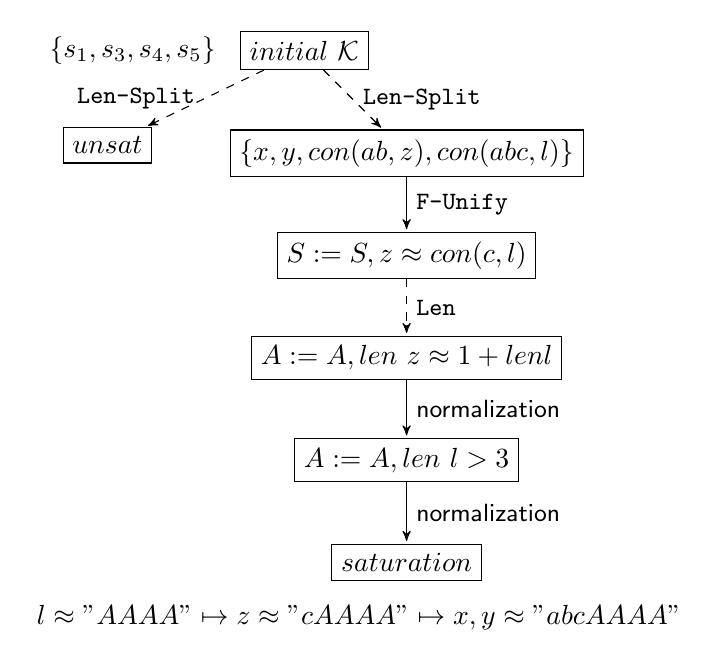
\begin{tikzpicture}[->,>=stealth',
		shorten >=1pt,auto,node distance=1.3cm,thin,
		main node/.style={rectangle,draw}, text node/.style={rectangle}]
		
		
		\node [left] at (-10mm,0) {$ \{s_1, s_3, s_4,  s_5\}$};
		\node[main node] (a) {$initial\ \mathcal{K}$};
		\node (dummy) [below of=a] {};
		%\node[main node] (b) [left of=dummy] {$unsat$};		
		\node [draw] (b) at (-25mm,-12mm)  {$unsat$};
		\node[main node] (c) [right of=dummy] {$\{ x,y,con(ab,z),con(abc,l)\}$};
		\node[main node] (d) [below of=c] {$S:=S, z \approx con(c, l)$};
		\node[main node] (e) [below of=d] {$A:=A, len\ z \approx 1 + len l$}; 
		\node[main node] (f) [below of=e] {$A:=A, len\ l > 3$};
		\node[main node] (g) [below of=f] {$saturation$};
		
		\node at (7mm,-72mm) {$ l \approx "AAAA" \mapsto z \approx "cAAAA" \mapsto x, y\approx "abcAAAA"$};
		
		\path[every node/.style={font=\sffamily\small}]
		(a) edge [dashed] node [left] {\texttt{Len-Split}} (b)
		(a) edge [dashed] node [right] {\texttt{Len-Split}} (c)
		(c) edge  node [right] {\texttt{F-Unify}} (d)
		(d) edge [dashed] node [right] {\texttt{Len}} (e)
		(e) edge  node [right] {normalization} (f)
		(f) edge  node [right] {normalization} (g);
		
		
		\end{tikzpicture}			
	\end{figure}	
}

\frame{
  \frametitle{Correctness}  
\begin{itemize}
\item  $Refutation\ Sound$: when the procedure answers with \texttt{unsat}, it can be trusted. 
\item  $Solution\ Sound$: when the procedure answers with \texttt{sat}, it can be trusted. 
\item $Solution\ Complete$: eventually get a model by finite model finding. 
\item $Refutation\ Complete$: the procedure may \underline{not} terminate for \texttt{unsat} problems.
\end{itemize}
}

\frame{
  \frametitle{Evaluation}  
\begin{itemize}
\item  There was an evaluation conducted by the authors with:
	\begin{description}
		\item[-] Z3-STR. 
		\item[-] Kaluza. 
	\end{description}
\item 50K benchmarks generated by Kudzu were used.
\item CVC4 string solver performed better. 
\item Since the string solver is natively integrated\end{itemize}
}
\frame{
  \frametitle{Observation}  
\begin{itemize}
	\item  Positive:.
\begin{itemize}
	\item  The idea of implementing the string solver \underline{natively} is unique.
	\item  This approach allowed \underline{high interaction} with core of cvc4.
	\item  Since it is \underline{not a plugin}, the performance is better than others.
	\item  This approach allowed uses of general purpose Arithmetic solver.
\end{itemize}

	\item  Negative:
\begin{itemize}
	\item  The application of the derivation rules is complicated.
	\item  Limited expressiveness, only supported few string methods.
\end{itemize}

\end{itemize}



}




\end{document}

